\section{USB board}

\subsection{Making connections}
Figure \ref{fig:panel_switch_wiring} shows how the front panel power
switch should be wired.

\begin{figure}[ht]
  \begin{center}
    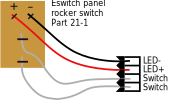
\includegraphics[clip,scale=1]{figs/panel_switch_wiring}
    \caption{Panel switch wiring \label{fig:panel_switch_wiring}}
  \end{center}
\end{figure}

Figure \ref{fig:post_cable} shows how to make the cable connecting the
monitored 3.3V output to the front panel binding posts.
\begin{figure}[ht]
  \begin{center}
    
\includegraphics[clip,scale=1]{figs/post_cable}
    \caption{Panel switch wiring \label{fig:post_cable}}
  \end{center}
\end{figure}


\clearpage{}
\subsection{Board checkout}


\subsubsection{Voltage rails}
Use table \ref{tab:usb_rails} to keep track of voltage rails.

\begin{table}[ht]
  \begin{center}
    \begin{tabular}{|c|c|c|c|}
      \hline
      Net name &Test points &Acceptable &Actual\\
      \hline \hline
      $\mathrm{V_{bus}}$ &TP100 vs.\ TP101 &\cwksentry{1in}{4.5V $\rightarrow$ 5.5V} 
        &\cwksentry{1in}{} \\
      \hline
      $\mathrm{+3.3V_{aux}}$ &TP400 vs.\ TP401 &\cwksentry{1in}{3.14V $\rightarrow$ 3.45V} 
        &\cwksentry{1in}{} \\
      \hline
      $\mathrm{+3.3V_{mon}}$ &TP500 vs.\ TP401 &\cwksentry{1in}{3.14V $\rightarrow$ 3.45V} 
        &\cwksentry{1in}{} \\
      \hline
    \end{tabular}
    \caption{Voltage rail checkout table for the USB
      board.\label{tab:usb_rails}}
  \end{center}
\end{table}

\subsubsection{Current monitor}
The current monitor output at J500 will have a fixed DC output, since
the voltage regulator following it always draws at least 1mA. As
illustrated in figure \ref{fig:monitor_test}, the slope set in
hardware should give $\Delta \mathrm{V_{out}}$ = 1V for each
additional 10mA of current draw from J501.  Since the voltage output
from J501 is controlled at 3.3V, a test load of 3.3k$\Omega$ should
increase the voltage at J500 by 100mV.

\begin{figure}[ht]
  \begin{center}
    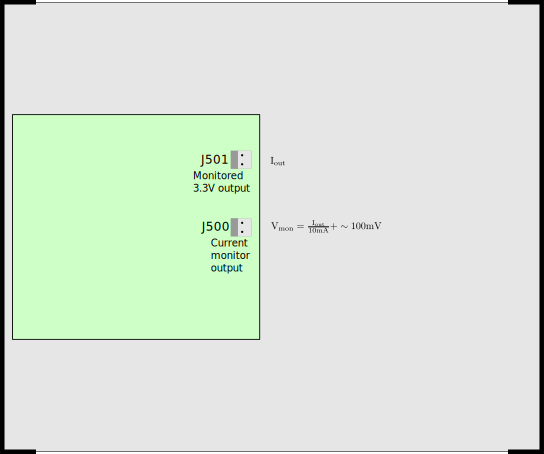
\includegraphics[clip,scale=.5]{figs/monitor_test}
    \caption{The output connectors used during the current monitor test.\label{fig:monitor_test}}
  \end{center}
\end{figure}

\begin{table}[ht]
  \begin{center}
    \begin{tabular}{|c|c|c|}
      \hline
      Load applied to J501 & Acceptable $\mathrm{V_{out}}$ at J500 & Measured $\mathrm{V_{out}}$ at J500\\
      \hline\hline
      Open                 &90mV $\rightarrow$ 110mV &\wksentry{2cm}{$\mathrm{V_{out,o}} =$}\\
      \hline
      3.3k$\Omega$         &\cwksentry{3cm}{$\mathrm{V_{out,o}}$ + 100mV} &\\
      \hline
    \end{tabular}
    \caption{Passing voltage measurements for the current monitor test.\label{tab:monitor_test}}
  \end{center}
\end{table}

\subsubsection{Serial loopback}
The serial loopback test is a basic test of the USB/serial interface
and the RS-232 transceiver.  Make the breakout cable shown in figure
\ref{fig:db9_breakout}, then make connections to the board as shown in
figure \ref{fig:serial_loopback}.

\begin{figure}[ht]
  \begin{center}
    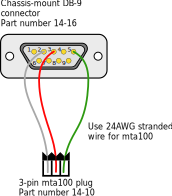
\includegraphics[clip,scale=1]{figs/usb_board_uart_to_db9}
    \caption{Wiring the DB9 breakout cable for the serial loopback
      test.\label{fig:db9_breakout}}
  \end{center}
\end{figure}

\begin{figure}[ht]
  \begin{center}
    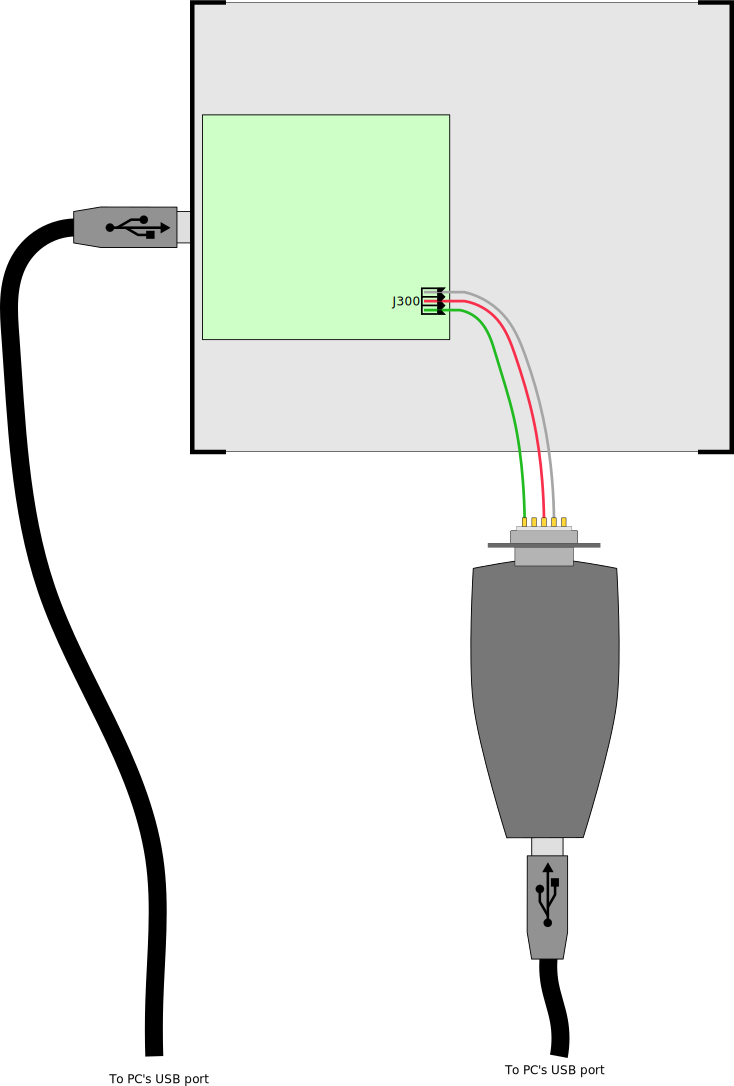
\includegraphics[clip,scale=0.5]{figs/serial_loopback_test}
    \caption{The setup for the serial loopback
      test.\label{fig:serial_loopback}}
  \end{center}
\end{figure}

The serial loopback test script is:
\begin{center}
  \texttt{boxcom/implement/data/scripts/tty\_loopback.py}
\end{center}
...and the test should pass at the speed listed in table
\ref{tab:loopback_test}.

\begin{table}[ht]
  \begin{center}
    \begin{tabular}{|c|c|}\hline
      Minimum passing baud  &Measured passing baud\\
      \hline\hline
      \cwksentry{5cm}{115200} &\cwksentry{5cm}{}\\
      \hline
    \end{tabular}
    \caption{Passing baud measurement for the serial loopback test.
      The usb board should be able to reliably pass the loopback test
      for data flowing in both directions at the minimum
      baud.\label{tab:loopback_test}}
  \end{center}
\end{table}
